\section{Force Cost Evaluation in a Tetrahedral Musculoskeletal System}

\subsection{Problem Statement}
The following triple integral represents the \textbf{force cost function} in a bounded musculoskeletal system with quadratic variation along the vertical axis:
$$\iiint_{E}(480.92x+592.03y+z^{2})dV$$
where $E$ is the solid tetrahedron bounded by: $x=0.1$, $y=0.3$, $z=0.4$, $x+y+z=5$. Evaluate the \textbf{total force cost} within the system.

\subsection{Detailed Solution}
\textit{ Sol. }
\begin{itemize}
	\item \textbf{Inner bounds ($z$):} $ x + y + z = 5 \Rightarrow z \in{[ 0.4,\ 5 - x - y ]} $
	\item \textbf{Middle bounds ($y$):} $ z_{\text{min}} = 0.4 \Rightarrow y \in{[ 0.3,\ 5 - 0.4 - x]} \iff y \in{[ 0.3,\ 4.6 - x]}  $
	\item \textbf{Outer bounds ($x$):} $ y_{\text{min}} = 0.3,\ z_{\text{min}} = 0.4 \Rightarrow x \in{[ 0.3,\ 5 - 0.3 - 0.4]} \iff x \in{[ 0.3,\ 4.3]} $
\end{itemize}

\begin{equation*}
	\begin{aligned}
		C & = \iiint_{E}(480.92x+592.03y+z^{2}) \, dV                                                                                            \\
		  & = \int_{0.1}^{4.3} \int_{0.3}^{4.6-x} \int_{0.4}^{5-x-y} (480.92x + 592.03y + z^2) \, dz \, dy \, dx                                 \\
		  & = \int_{0.1}^{4.3} \int_{0.3}^{4.6-x} \left[ (480.92x + 592.03y)z + \frac{z^3}{3} \right]_{0.4}^{5-x-y} \, dy \, dx                  \\
		  & = \int_{0.1}^{4.3} \int_{0.3}^{4.6-x} \Bigg( (480.92x + 592.03y)(4.6-x-y)                                                            \\
		  & \qquad\qquad + \frac{(5-x-y)^3}{3} - \frac{0.064}{3} \Bigg) \, dy \, dx                                                              \\
		  & = \int_{0.1}^{4.3} \Bigg[ 480.92x \left((4.6-x)y - \frac{y^2}{2}\right) + 592.03 \left( \frac{(4.6-x)y^2}{2} - \frac{y^3}{3} \right) \\
		  & \qquad\qquad - \frac{(5-x-y)^4}{12} - \frac{0.064y}{3} \Bigg]_{y=0.3}^{y=4.6-x} \, dx                                                \\
		  & = \int_{0.1}^{4.3} \Bigg( 240.46x(4.6-x)^2 + \frac{592.03}{6}(4.6-x)^3 - \frac{0.064(4.6-x)}{3} - \frac{0.4^4}{12}                   \\
		  & \qquad\qquad - 480.92x(1.335 - 0.3x) - 592.03(0.045(4.6-x) - 0.009) + \frac{(4.7-x)^4}{12} + 0.0064 \Bigg) \, dx                     \\
		  & = \Bigg[ 240.46\left(\frac{x^4}{4} - \frac{9.2x^3}{3} + \frac{21.16x^2}{2}\right) - \frac{592.03(4.6-x)^4}{24}                       \\
		  & \qquad\qquad + \frac{0.04(4.6-x)^2}{6} - \frac{0.0256x}{12} - 480.92\left(\frac{1.335x^2}{2} - \frac{0.3x^3}{3}\right)               \\
		  & \qquad\qquad + \frac{26.64135(4.6-x)^2}{2} + 5.32827x - \frac{(4.7-x)^5}{60} + 0.0064x \Bigg]_{0.1}^{4.3}                            \\
		  & \approx \boxed{16,732.3117}
	\end{aligned}
	\label{eq:stu4q5}
\end{equation*}

\subsection{Matlab Implementation}
\begin{figure}[H]
	\begin{center}
		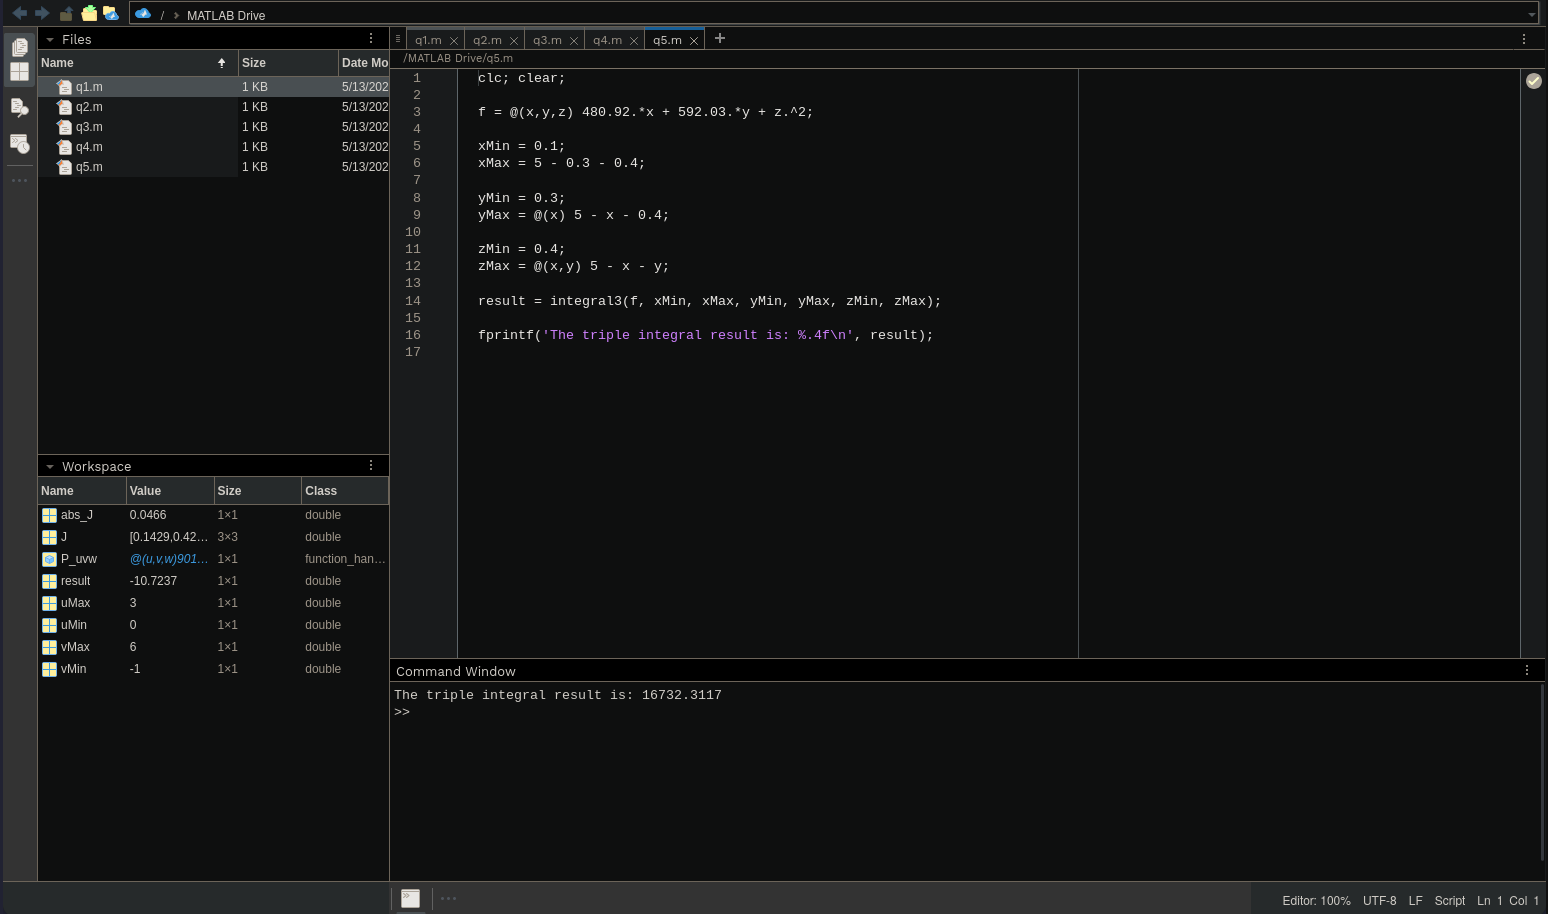
\includegraphics[width=0.95\textwidth]{figures/stu4q5.png}
	\end{center}
	\caption{Student 04 - Matlab Screenshot}
	\label{fig:stu4q5}
\end{figure}

\subsection{Conclusion}
The integration over the tetrahedral region (Equation \ref{eq:stu4q5}) results in the \textbf{same} value as the MATLAB script (Figure \ref{fig:stu4q5}).
